\documentclass[../delivery_hospital_report.tex]{subfiles}
\graphicspath{ {images/}{../images/}{../../images/} }
\begin{document}


\section{Interface com Usuário}
\subsection{Placa}

%================================ INTERFACE COM USUARIO PROTÓTIPO ========================
\subsubsection{Protótipo}

\paragraph{Esquemático}

\begin{figure}[h]
\centering
    \caption{Protótipo placa de Interface com Usuário - Esquemático principal }
    \centering % para centralizarmos a figura
    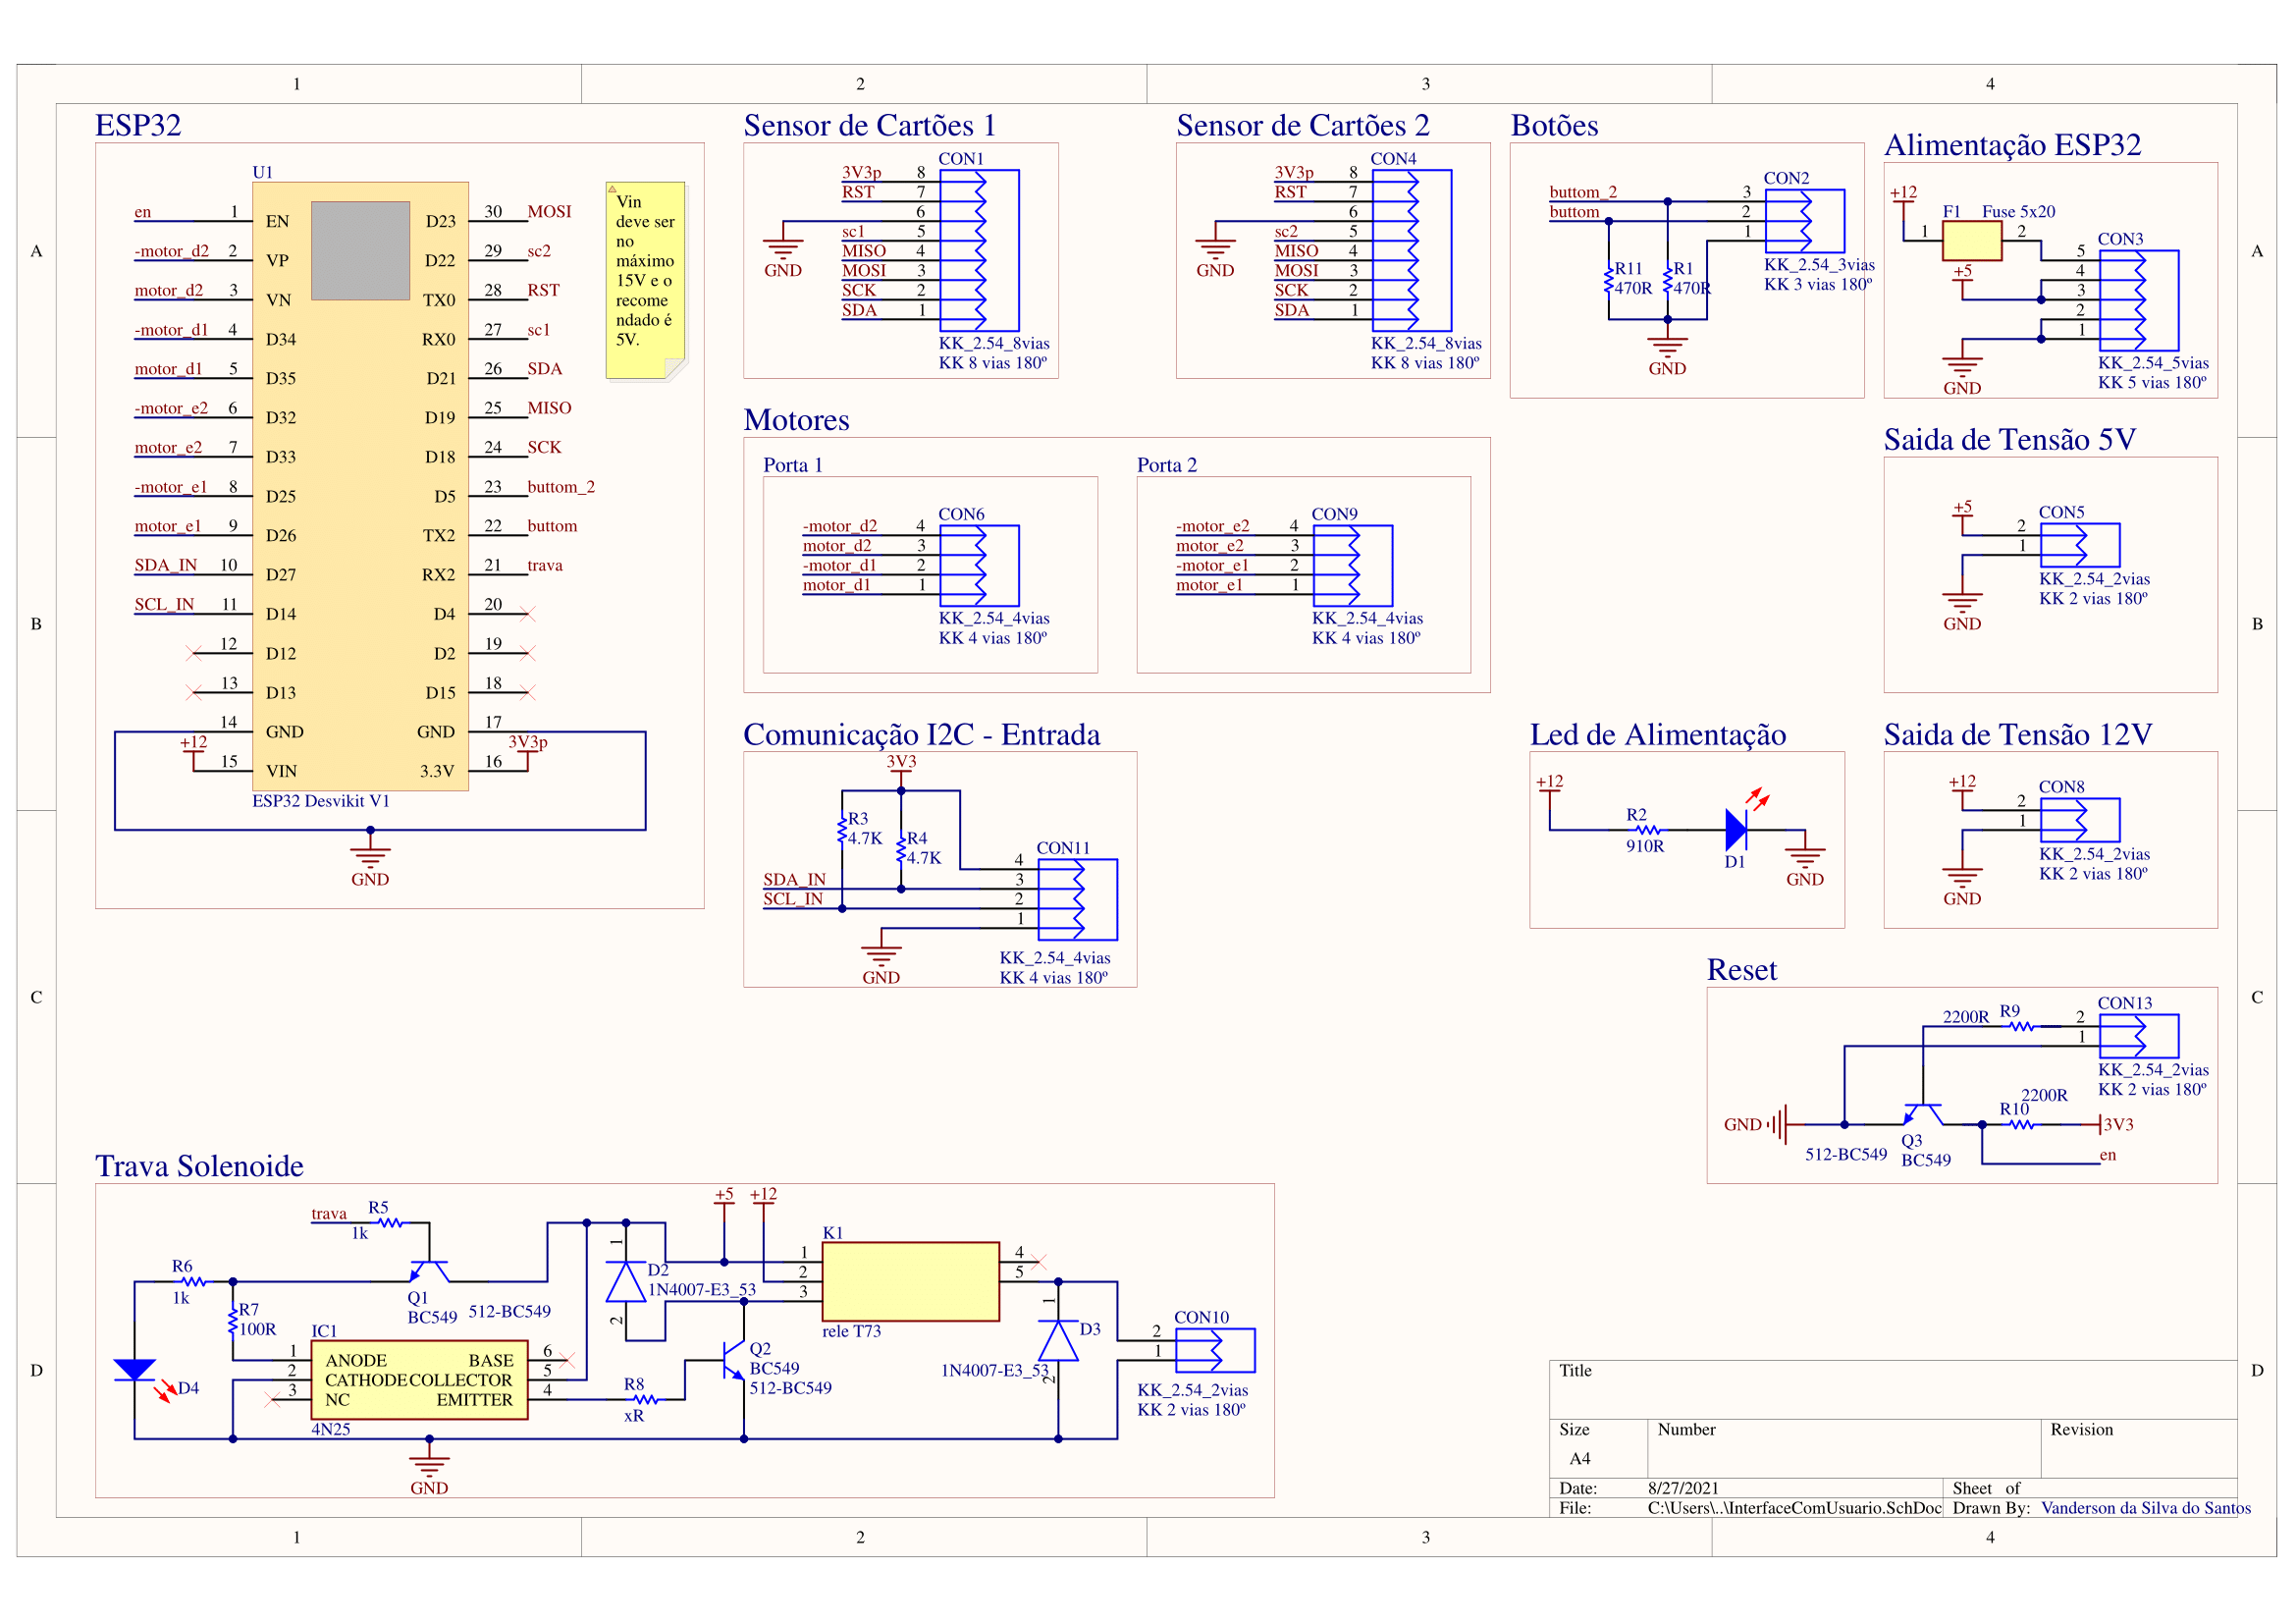
\includegraphics[width=17cm]{modulos/InterfaceComUsuario-1.png}
    \caption*{Fonte: Elaborado pelo autor no software Altium Design\cite{altium21} }
    \label{Protótipo placa de ## - Esquemático principal}
\end{figure}

\begin{table}[]
\caption{Componentes Utilizados na placa de Interface com Usuário - Protótipo}
\centering
\begin{adjustbox}{width=\columnwidth,center}
\begin{tabular}{|c|c|c|c|c|}
\hline
Component                   & Description                                    & Designator                             & Footprint                   & Quantity \\ \hline
KK\_2.54\_8vias             & Conector KK 2.54mm 8   vias                    & CON1, CON4                             & KK\_8vias\_180°             & 2        \\ \hline
KK\_2.54\_3vias             & Conector KK 2.54mm 3   vias                    & CON2                                   & KK\_3vias\_180º             & 1        \\ \hline
KK\_2.54\_5vias             & Conector KK 2.54mm 5   vias                    & CON3                                   & KK\_5vias\_180°             & 1        \\ \hline
KK\_2.54\_2vias             & Conector KK 2.54mm 2   vias                    & CON5, CON8, CON10,   CON13             & KK\_2VIAS\_180º             & 4        \\ \hline
KK\_2.54\_4vias             & Conector KK 2.54mm 4   vias                    & CON6, CON9, CON11                      & KK\_4vias\_180°             & 3        \\ \hline
LED 5MM RED                 & LED 5MM RED                                    & D1, D4                                 & LED 5MM RED                 & 2        \\ \hline
1N4007-E3\_53               & Diode                                          & D2, D3                                 & DIOAD1405W89L465D235        & 2        \\ \hline
Fuse 5x20                   & Fuse                                           & F1                                     & Fuse 5x20                   & 1        \\ \hline
4N25                        & Integrated Circuit                             & IC1                                    & DIP762W50P254L712H450Q6N    & 1        \\ \hline
rele T73                    & Relay or Contactor                             & K1                                     & JQC3FT731Z12VDC             & 1        \\ \hline
BC549                       & TRANS NPN 30V 0.1A   TO-92                     & Q1, Q2, Q3                             & TO92                        & 3        \\ \hline
RES 470R 1/4W   CARBON FILM & RES 470R OHM 1/4W 5\%   CARBON FILM            & R1, R2, R5, R6, R7,   R8, R9, R10, R11 & RES 470R 1/4W CARBON   FILM & 9        \\ \hline
4.7K                        & RES 4.7K OHM 1/4W 5\%   CARBON FILM            & R3, R4                                 & RES 4.7K 1/4W CARBON   FILM & 2        \\ \hline
microcontrolador            & microcontrolador com   moculo bluethoth e wifi & U1                                     & ESP32\_Desvikit\_v1         & 1        \\ \hline

\end{tabular}
\end{adjustbox}
\centering
\caption*{Fonte: Elaborado pelo autor}
\label{table:voc}
\end{table}


\paragraph{Printed Circuit board (PCB)}

\begin{figure}[!ht]
    \centering
    \begin{minipage}{0.5\textwidth}
        \centering
        \caption{Protótipo Interface com Usuário - PCB 2D}
        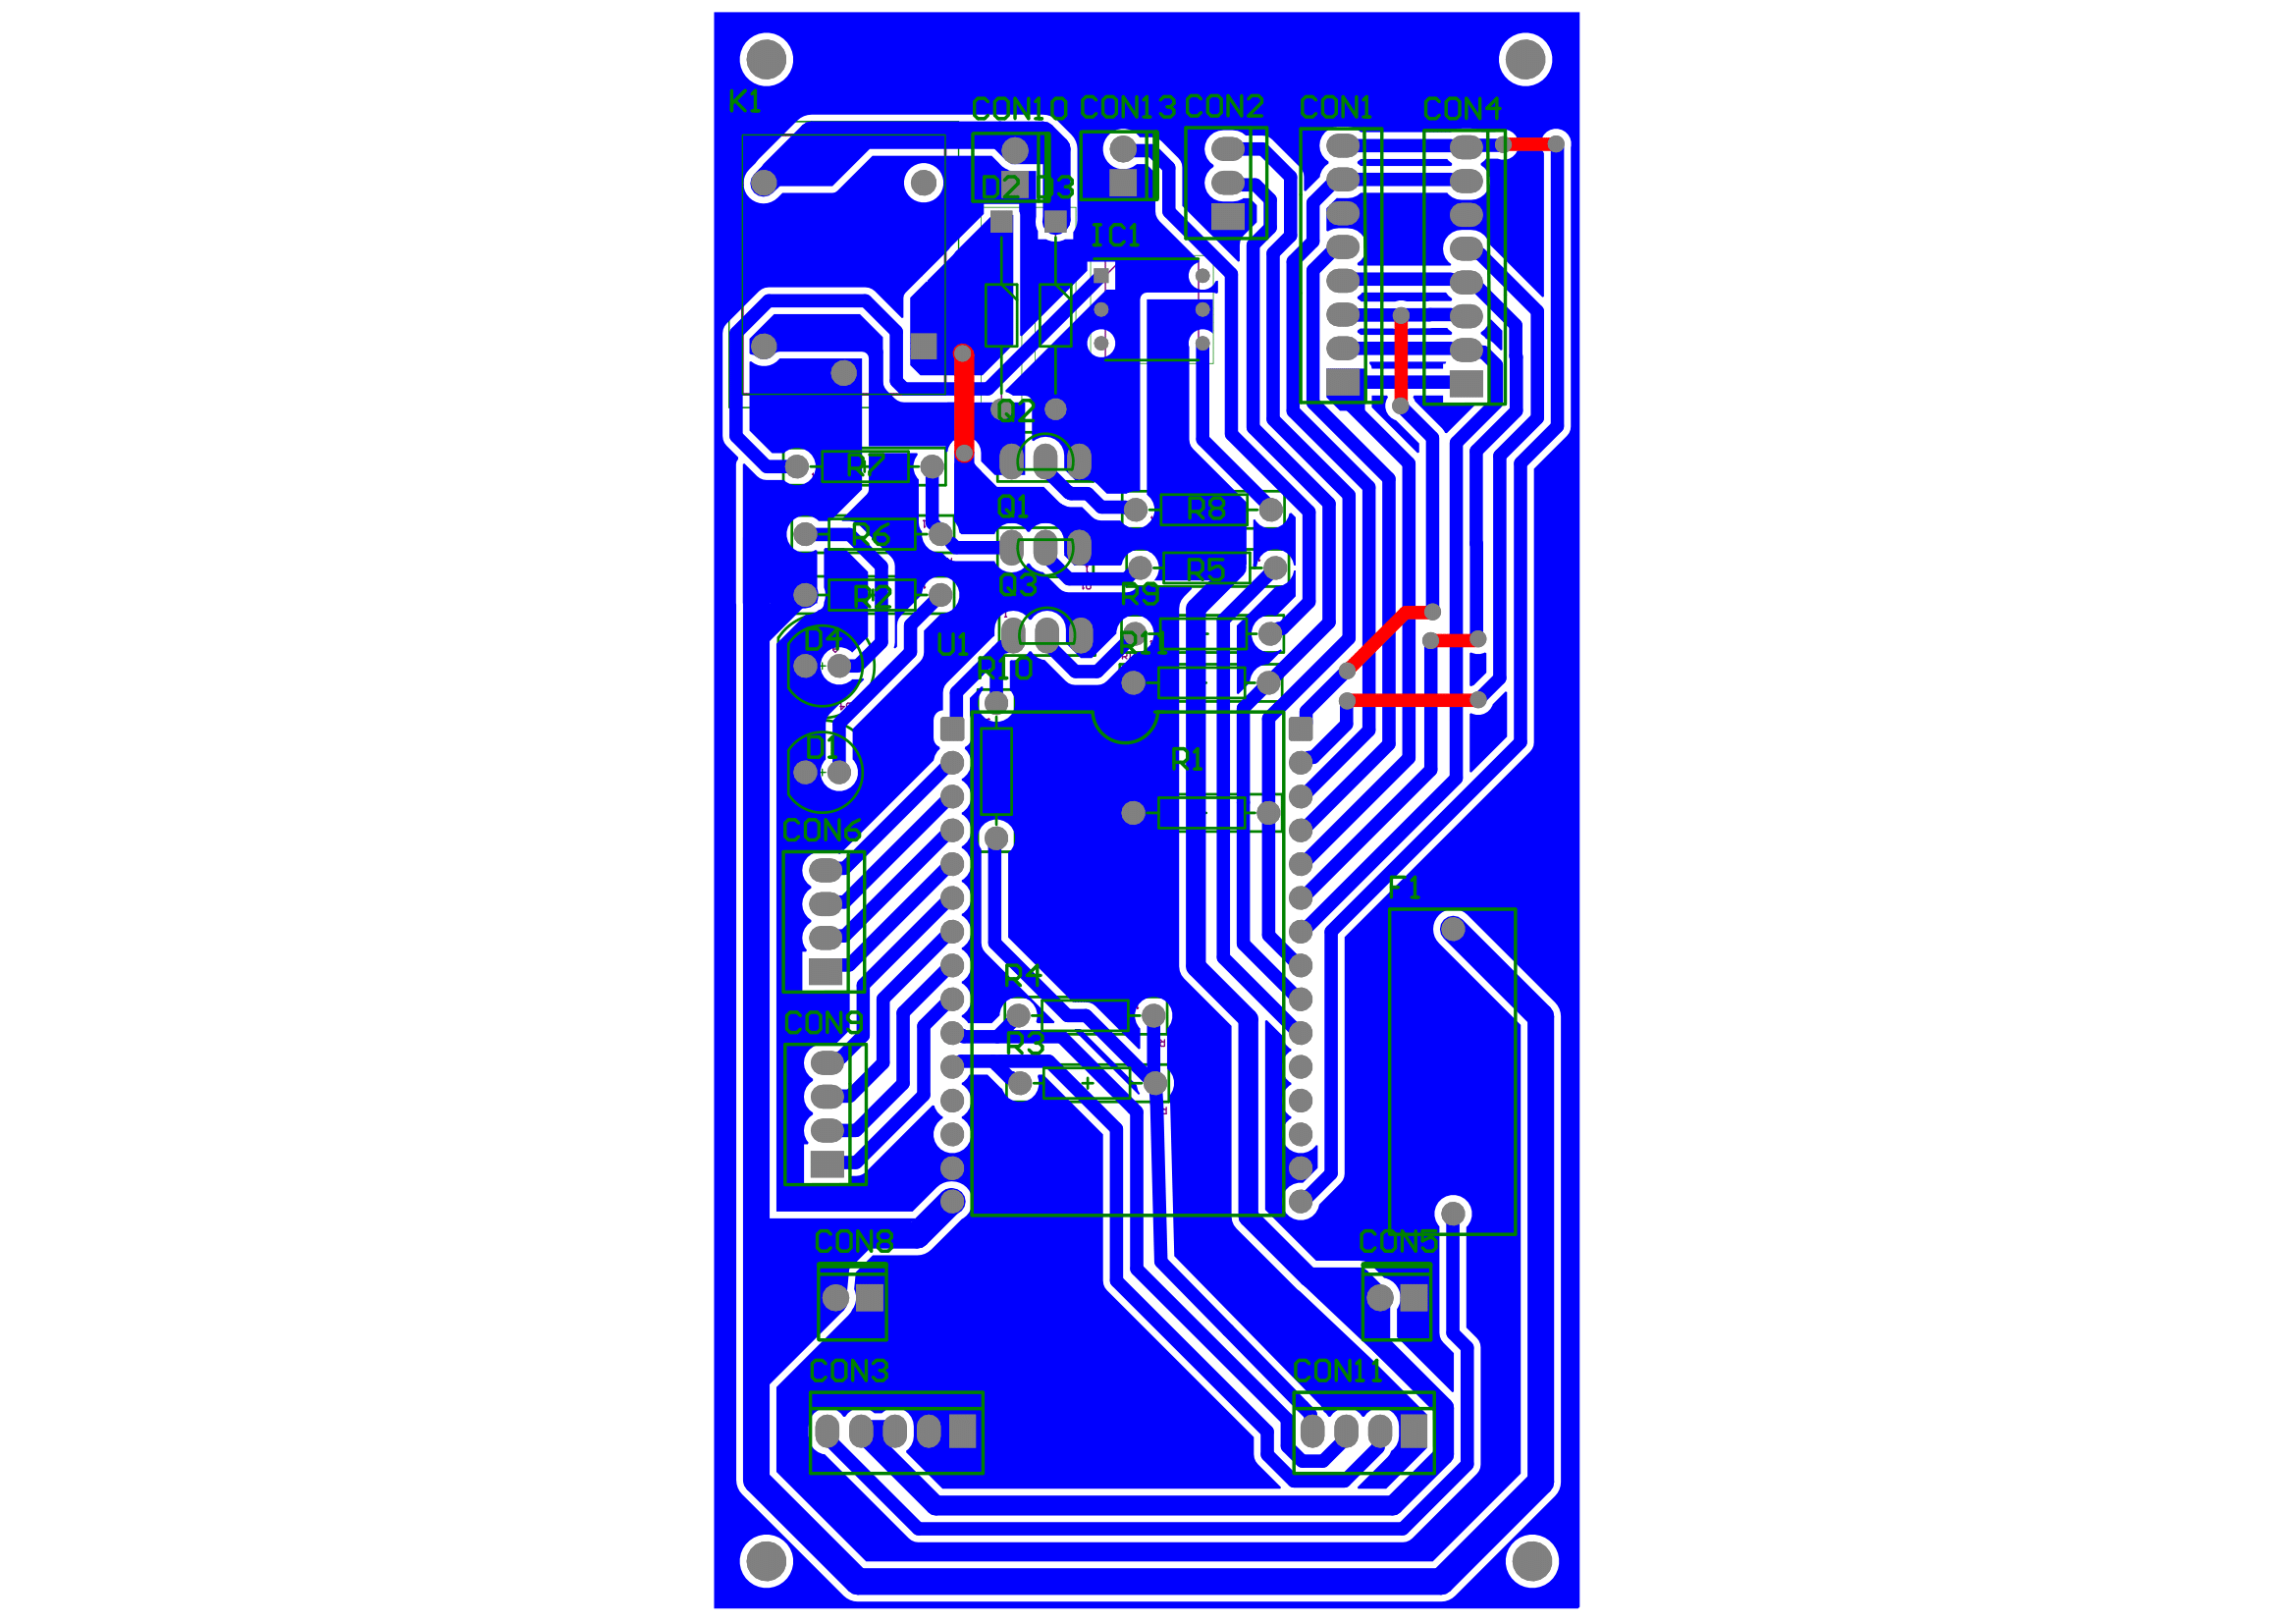
\includegraphics[width=1.03\textwidth]{modulos/InterfaceComUsuario-2.png} 
        \label{fig:figura1minipg}
    \end{minipage}\hfill
    \begin{minipage}{0.5\textwidth}
        \centering
        \caption{Protótipo Interface com Usuário - PCB 3D }
        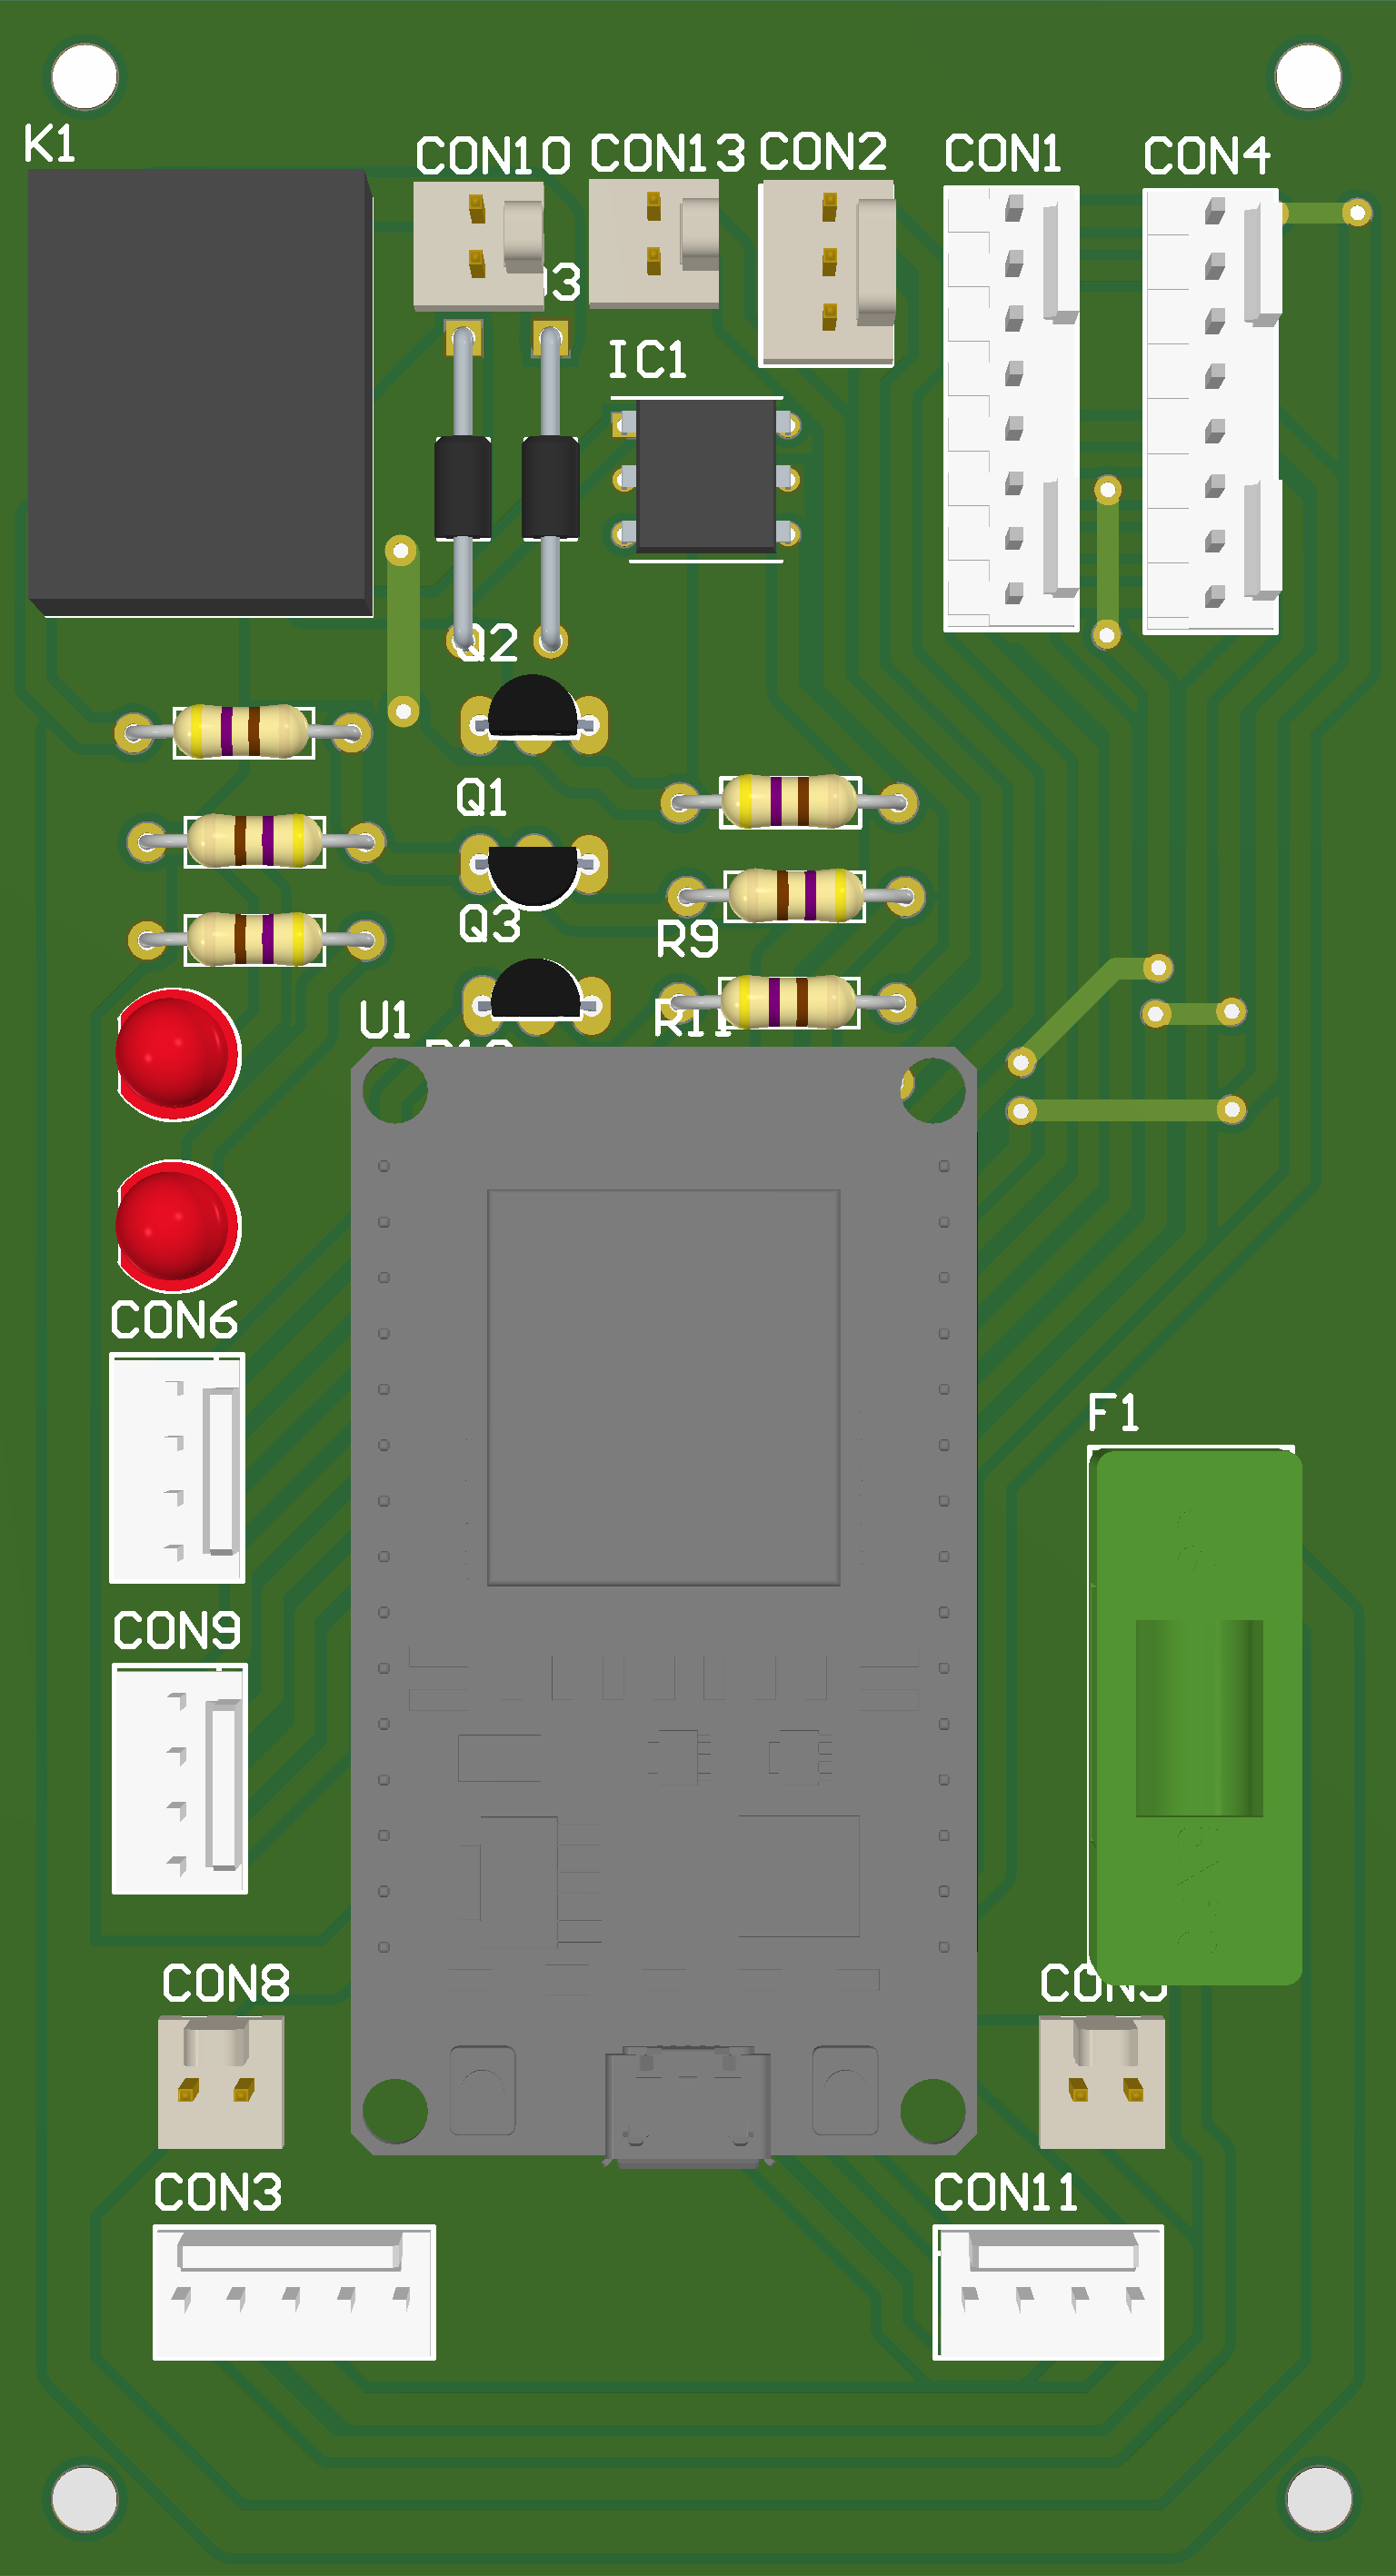
\includegraphics[width=0.4\textwidth]{modulos/InterfaceComUsuario.png} 
        \label{fig:figura1minipg}
    \end{minipage}\hfill
    
    \caption*{Fonte: Elaborado pelo autor no software Altium Design\cite{altium21} }
    \label{fig:figurasminipg}
\end{figure}

\begin{figure}[!ht]
    \centering
    \begin{minipage}{0.5\textwidth}
        \centering
        \caption{Protótipo Interface com Usuário - Trilhas}
        \includegraphics[width=0.8\textwidth]{example-image-a} 
        \label{fig:figura1minipg}
    \end{minipage}\hfill
    \begin{minipage}{0.5\textwidth}
        \centering
        \caption{Protótipo Interface com Usuário - Completa }
        \includegraphics[width=0.8\textwidth]{example-image-a} 
        \label{fig:figura1minipg}
    \end{minipage}\hfill
    \caption*{Fonte: Elaborado pelo autor }
    \label{fig:figurasminipg}
\end{figure}

%================================ INTERFACE COM USUARIO OFICIAL ========================
\subsubsection{Oficial}

\paragraph{Esquemático}

\begin{figure}[h]
\centering
    \caption{placa de Interface com Usuário - Esquemático principal }
    \centering % para centralizarmos a figura
    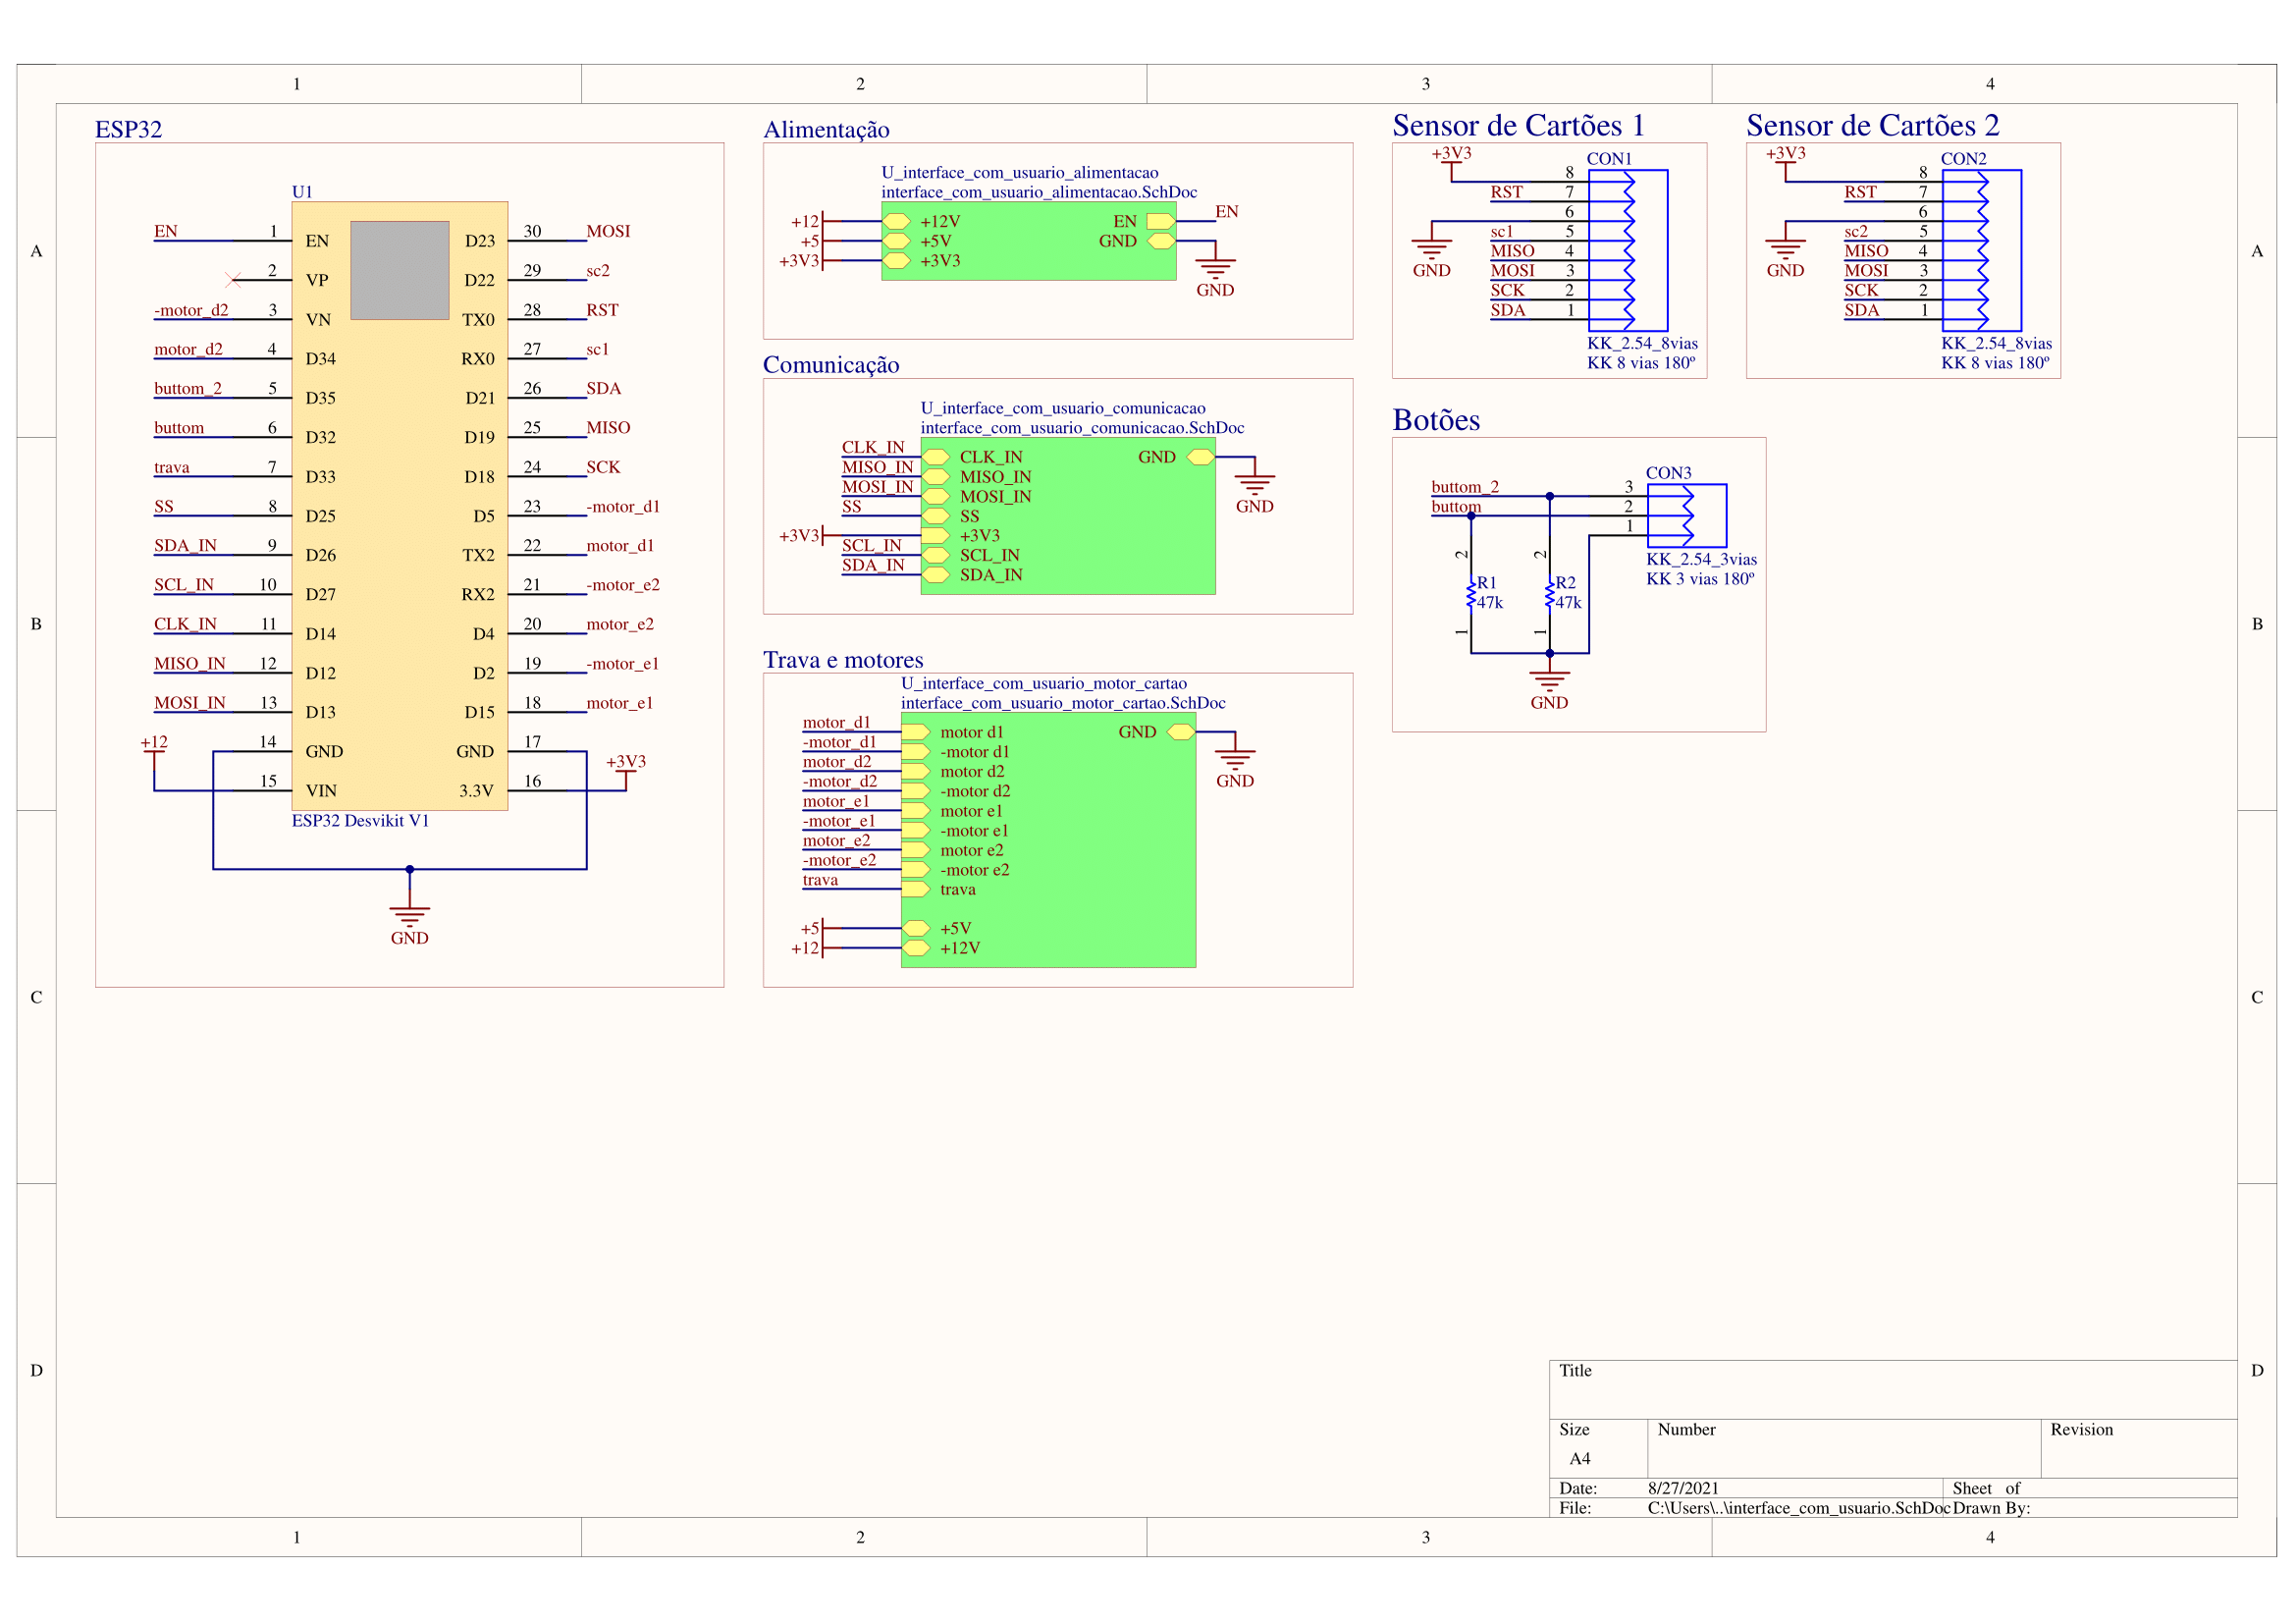
\includegraphics[width=17cm]{modulos/interface_com_usuario-1.png}
    \caption*{Fonte: Elaborado pelo autor no software Altium Design\cite{altium21} }
    \label{Protótipo placa de ## - Esquemático principal}
\end{figure}

\begin{table}[]
\caption{Componentes Utilizados na placa de Interface com Usuário}
\centering
\begin{adjustbox}{width=\columnwidth,center}
\begin{tabular}{|c|c|c|c|c|}

\hline
Component        & Description                                    & Designator                                                           & Footprint           & Quantity \\ \hline
KK\_2.54\_8vias  & Conector KK 2.54mm 8   vias                    & CON1, CON2                                                           & KK\_8vias\_180°     & 2        \\ \hline
KK\_2.54\_3vias  & Conector KK 2.54mm 3   vias                    & CON3                                                                 & KK\_3vias\_180º     & 1        \\ \hline
KK\_2.54\_2vias  & Conector KK 2.54mm 2   vias                    & \begin{tabular}[c]{@{}l@{}}CON4, CON6, \\ CON7,   CON12\end{tabular} & KK\_2VIAS\_180º     & 4        \\ \hline
KK\_2.54\_6vias  & Conector KK 2.54mm 6   vias                    & CON5                                                                 & KK\_6vias\_180°     & 1        \\ \hline
KK\_2.54\_5vias  & Conector KK 2.54mm 5   vias                    & CON8                                                                 & KK\_5vias\_180°     & 1        \\ \hline
KK\_2.54\_4vias  & Conector KK 2.54mm 4   vias                    & CON9, CON10, CON11                                                   & KK\_4vias\_180°     & 3        \\ \hline
LED 3MM RED      & LED 3MM RED                                    & D1                                                                   & LED RED             & 1        \\ \hline
1N4007 smd       & Diode smd                                      & D2, D3                                                               & DIOM5327X242N       & 2        \\ \hline
rele T73         & Relay or Contactor                             & K1                                                                   & JQC3FT731Z12VDC     & 1        \\ \hline
Trans BC817      & Transistor BJT NPN   BC817-25-7-F              & Q1, Q2, Q4                                                           & SOT96P240X110-3N    & 3        \\ \hline
4N25-X007T       & Phototransistor                                & Q3                                                                   & SOP254P1030X440-6N  & 1        \\ \hline
47k              & RES 1206 5\%                                   & R1, R2                                                               & RESC3216X60N        & 2        \\ \hline
680R             & Resistor                                       & R3                                                                   & RESC3216X60N        & 1        \\ \hline
2k2              & Resistor                                       & R4, R5                                                               & RESC3216X60N        & 2        \\ \hline
4k7              & RES 1206 5\%                                   & R6, R7                                                               & RESC3216X60N        & 2        \\ \hline
1k               & RES 1206 5\%                                   & R8, R10                                                              & RESC3216X60N        & 2        \\ \hline
100R             & RES 1206 5\%                                   & R9                                                                   & RESC3216X60N        & 1        \\ \hline
microcontrolador & microcontrolador com   moculo bluethoth e wifi & U1                                                                   & ESP32\_Desvikit\_v1 & 1        \\ \hline

\end{tabular}
\end{adjustbox}
\centering
\caption*{Fonte: Elaborado pelo autor}
\label{table:voc}
\end{table}

%================================ INTERFACE COM USUARIO FIRMWARE ========================
\subsection{Firmware}

\end{document}